\documentclass[11pt, a4paper]{article}

\usepackage{pdfpages}
\usepackage{parallel}
\usepackage[T2A]{fontenc}
\usepackage{ucs}
\usepackage[utf8x]{inputenc}
\usepackage[polish,english,russian]{babel}
\usepackage{hyperref}
\usepackage{rotating}
\usepackage[inner=2cm,top=1.8cm,outer=2cm,bottom=2.3cm,nohead]{geometry}
\usepackage{listings}
\usepackage{graphicx}
\usepackage{wrapfig}
\usepackage{longtable}
\usepackage{indentfirst}
\usepackage{array}
\usepackage{tikzsymbols}
\usepackage{soul}
\usepackage[ruled,vlined]{algorithm2e}
%\counterwithout{figure}{section} 

\usepackage{url}
\makeatletter
\g@addto@macro{\UrlBreaks}{\UrlOrds}
\makeatother

\newcolumntype{P}[1]{>{\raggedright\arraybackslash}p{#1}}
\frenchspacing
\usepackage{fixltx2e} %text sub- and superscripts
\usepackage{icomma} % коскі ў матэматычным рэжыме
\PreloadUnicodePage{4}

\newcommand{\longpage}{\enlargethispage{\baselineskip}}
\newcommand{\shortpage}{\enlargethispage{-\baselineskip}}

\def\switchlang#1{\expandafter\csname switchlang#1\endcsname}
\def\switchlangbe{
\let\saverefname=\refname%
\def\refname{Літаратура}%
\def\figurename{Іл.}%
}
\def\switchlangen{
\let\saverefname=\refname%
\def\refname{References}%
\def\figurename{Fig.}%
}
\def\switchlangru{
\let\saverefname=\refname%
\let\savefigurename=\figurename%
\def\refname{Литература}%
\def\figurename{Рис.}%
}

\hyphenation{admi-ni-stra-tive}
\hyphenation{ex-pe-ri-ence}
\hyphenation{fle-xi-bi-li-ty}
\hyphenation{Py-thon}
\hyphenation{ma-the-ma-ti-cal}
\hyphenation{re-ported}
\hyphenation{imp-le-menta-tions}
\hyphenation{pro-vides}
\hyphenation{en-gi-neering}
\hyphenation{com-pa-ti-bi-li-ty}
\hyphenation{im-pos-sible}
\hyphenation{desk-top}
\hyphenation{elec-tro-nic}
\hyphenation{com-pa-ny}
\hyphenation{de-ve-lop-ment}
\hyphenation{de-ve-loping}
\hyphenation{de-ve-lop}
\hyphenation{da-ta-ba-se}
\hyphenation{plat-forms}
\hyphenation{or-ga-ni-za-tion}
\hyphenation{pro-gramming}
\hyphenation{in-stru-ments}
\hyphenation{Li-nux}
\hyphenation{sour-ce}
\hyphenation{en-vi-ron-ment}
\hyphenation{Te-le-pathy}
\hyphenation{Li-nux-ov-ka}
\hyphenation{Open-BSD}
\hyphenation{Free-BSD}
\hyphenation{men-ti-on-ed}
\hyphenation{app-li-ca-tion}

\def\progref!#1!{\texttt{#1}}
\renewcommand{\arraystretch}{2} %Іначай формулы ў матрыцы зліпаюцца з лініямі
\usepackage{array}

\def\interview #1 (#2), #3, #4, #5\par{

\section[#1, #3, #4]{#1 -- #3, #4}
\def\qname{LVEE}
\def\aname{#1}
\def\q ##1\par{{\noindent \bf \qname: ##1 }\par}
\def\a{{\noindent \bf \aname: } \def\qname{L}\def\aname{#2}}
}

\def\interview* #1 (#2), #3, #4, #5\par{

\section*{#1\\{\small\rm #3, #4. #5}}
\ifx\ParallelWhichBox\undefined%
    \addcontentsline{toc}{section}{#1, #3, #4}%
\else%
\ifnum\ParallelWhichBox=0%
    \addcontentsline{toc}{section}{#1, #3, #4}%
\fi\fi%

\def\qname{LVEE}
\def\aname{#1}
\def\q ##1\par{{\noindent \bf \qname: ##1 }\par}
\def\a{{\noindent \bf \aname: } \def\qname{L}\def\aname{#2}}
}

\newcommand{\interviewfooter}[1]{
\vskip 1em
\noindent \textit{#1}
}

%\twocolumn
\begin{document}

\title{Механические мыши}
\author{Общая информация}
\date{}
\maketitle

Для отслеживания движения механические мыши используют колеса или шарик, преобразуя их линейного движения по поверхности во вращательное движение коммутаторов или датчиков вращения ролика.

\begin{figure}[h]
    \centering
    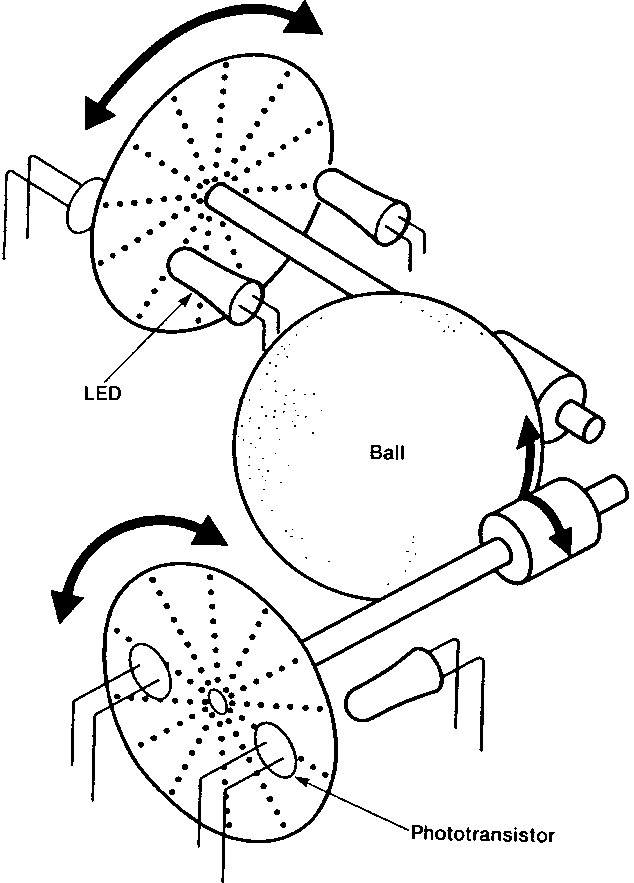
\includegraphics[width=0.3\linewidth]{theory_mech/2.1.png}
    \caption{Механическая мышь с шариком и роликами}
    \label{fig:theoryBallOpt}
\end{figure}

\begin{figure}[h]
    \centering
    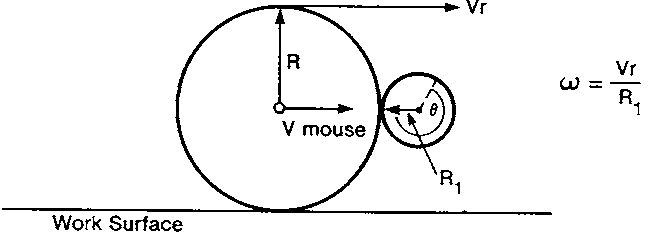
\includegraphics[width=0.3\linewidth]{theory_mech/2.2.png}
    \caption{Шар и ролик}
    \label{fig:theoryBallRoll}
\end{figure}

Мыши, которые используют шар для определения движения, могут быть представлены системой, показанной на рисунке \ref{fig:theoryBallRoll}. Скорость окружности шара $V_r$, равна скорости мыши, $V$. Так как ролик не прикреплен непосредственно к оси шара, а опирается на его окружность, при условии отсутствия проскальзывания скорость окружности ролика равна скорости окружности шара. Угловая скорость и вращение ролика теперь связаны с движением мыши с помощью приведенных выше уравнений, но радиус $R$ теперь намного меньше, и вал вращается намного быстрее.

$$\omega = V/R_1$$

\noindent где $V$ -- скорость мыши, а $R_1$ -- радиус ролика. Поскольку ролик меньше радиусом, он вращается быстрее при заданной скорости мыши.

Движение передается на датчики следующим образом. Ролики, которые прямо или косвенно вращаются колесом или шаром, подключены непосредственно к датчикам движения.

%\section{Оптомеханические мыши} \label{title:OptoMechanical}

Оптомеханические мыши для генерации квадратурных сигналов A и B используют устройство, называемое оптическим прерывателем. Как показано на рисунке \ref{fig:theoryQuadEncoder}, оптомеханическая система состоит из источника света (обычно светодиода), фотоприемника и оптического прерывателя, который соединен с вращающимся роликом мыши.

Прерыватель имеет серию чередующихся черных и белых полос, которые позволяют свету от светодиода попадать на детектор. Поскольку прерыватель вращается поперек линии светового луча, сплошные сегменты, расположенные между щелями, будут прерывать луч, и на выходе детектора появится серия импульсов напряжения. Второй квадратурный выход получается при использовании второго светодиода и детектора, которые смещены относительно первого светодиода и детектора на одну четверть угла радиальных прорезенй, или при использовании прорезей, которые смещены на одну четверть их периода, аналогично смещенным проводящим сегментам коммутатора. Маска с двумя сквозными отверстиями может использоваться с коммутатором, чтобы световые лучи находились в квадратуре относительно вращения прерывателя. Маска может быть просверлена или выполнена методом литья так, чтобы отверстия различались по фазе точно на 90 градусов.

\begin{figure}[h]
    \centering
    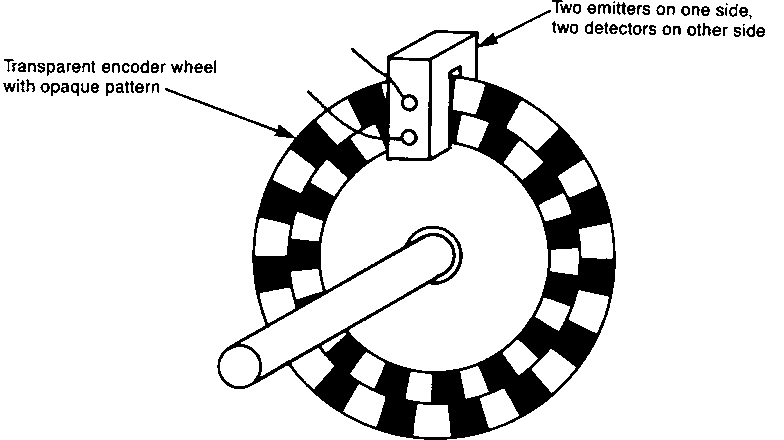
\includegraphics[width=0.5\linewidth]{theory_mech/2.76.PNG}
    \caption{Оптический энкодер с квадратурными выходами}
    \label{fig:theoryQuadEncoder}
\end{figure}

\begin{figure}[h]
    \centering
    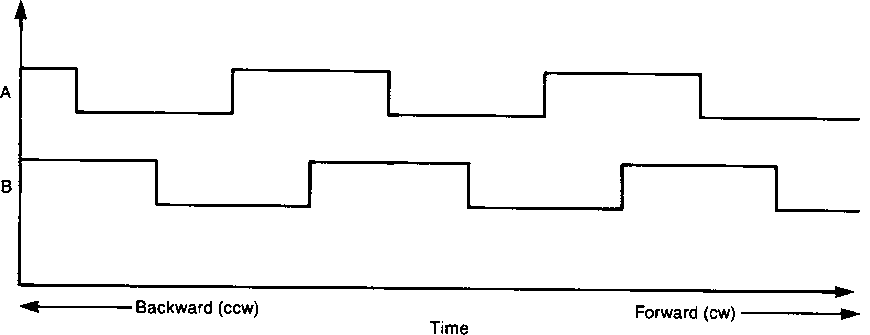
\includegraphics[width=0.5\linewidth]{theory_mech/2.77.PNG}
    \caption{Квадратурные сигналы}
    \label{fig:theoryQuadDiag}
\end{figure}

Выход оптического энкодера представляет собой два квадратурных сигнала, как показано на рисунке \ref{fig:theoryQuadDiag}. Направление можно определить, изучив соотношение фаз двух сигналов. Если сигнал A находится в состоянии высокого уровня, когда на сигнале B возникает восходящий фронт, то движение происходит в прямом направлении. Если микропроцессор достаточно быстр, сигналы могут быть подключены непосредственно к входному порту, а все декодирование и подсчет выполняются в программном обеспечении.

\end{document}
